\documentclass[FIPLY_base.tex]{subfiles}

%\author{Daniel Bersenkowitsch}
	
\begin{document}
	\subsection{Trainingsplan}
		Der Trainingsplan ist das Herzstück des Projekts. Wie in der Theorie beschrieben wird dieser mittels eines Algorithmus umgesetzt. 
	\subsubsection{Die Ansicht}
		 In der Trainingsplan Ansicht kann der Benutzer seine Trainingspläne verwalten.
		 \begin{figure}[H]
			\begin{subfigure}[b]{0.4\textwidth}
				In der obigen Leiste befinden sich die Optionen \grqq{}hinzufügen\grqq{}, \grqq{}löschen\grqq{}, und die Knöpfe zum Exportieren eines ausgewählten Plans.\newline
				Unterhalb ist eine ListView mit den existierenden Trainingsplänen. Es kann immer nur ein Plan gleichzeitig ausgewählt werden. Der Plan der ausgewählt ist, wird in dr Trainingssession herangezogen. Als additionalen Informationen stehen unterhalb des Trainingsplannamens dessen Trainingsziel und Anfang- und Enddatum.
				Beim Löschen eines Trainingsplan  bittet die Applikation vohe um eine Bestätigung.
				\newline\newline\newline\newline
			\end{subfigure}
			\hfil
		 	\begin{subfigure}[b]{0.4\textwidth}
		 		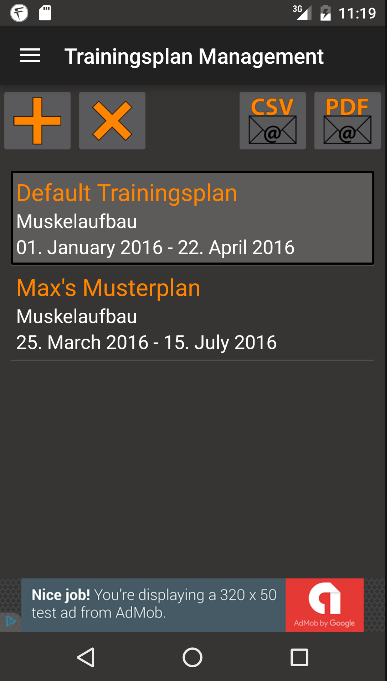
\includegraphics[scale=0.50]{img/tplanmgmt}
		 		\caption{Ansicht des Trainingspläne}
		 	\end{subfigure}
		 \end{figure}
	\newpage
	\subsubsection{Das Erstellen}
	Um einen neuen Trainingsplan zu Erstellen drückt man auf den Plus-Knopf ganz links in der Ansichtsleiste. Man wird zur Erstellungsansicht weitergeleitet die folgens aussieht:
	\begin{figure}[H]
		\begin{subfigure}[b]{0.5\textwidth}
			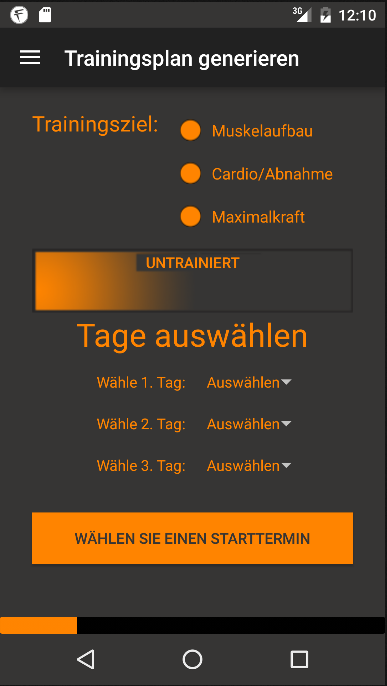
\includegraphics[scale=0.5]{img/generieren1}
			\caption{Trainingsplan erstellen: unausgefülltes Formular}
		\end{subfigure}
		\begin{subfigure}[b]{0.5\textwidth}
			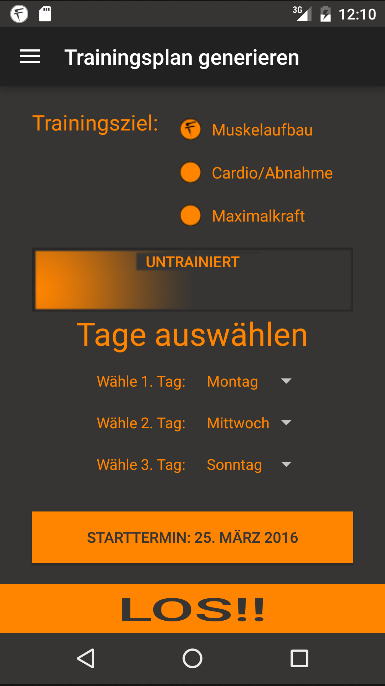
\includegraphics[scale=0.5]{img/generieren2}
			\caption{Trainingsplan erstellen: ausgefülltes Formular}
		\end{subfigure}
	\end{figure}
	\ \\
	Der Benutzer wählt nun aus, welches Trainingsziel er verfolgen will. Weiters kann er seine Einstellung ändern, ob er trainiert oder untrainiert ist. Danach wählt man 3 Trainingstage aus, an denen man trainieren will. Die jeweiligen Übungen werden dann auf diese Tage verteilt. Gleichzeitig, während des Ausfüllens des Formulars bewegt sich eine ProgressBar mit, die sich je mehr füllt, desto mehr Informationen eingegeben worden sind. Bei einer Füllung von 100 Prozent erscheint der \grqq{}LOS!!\grqq{}-Knopf, mit denen das Generieren gestartet werden kann. 
	\begin{figure}[H]
		\begin{subfigure}[b]{0.4\textwidth}
			Nach der Betätigung dieses Knopfes wird man wieder zur Trainingsplanübersicht gebracht, wo sich der neuerstellte Plan befindet. Ab dem Startdatum kann der Plan dann in der Trainingssession in Verwendung gebracht werden.
			\newline
		\end{subfigure}
		\hfil
		\begin{subfigure}[b]{0.5\textwidth}
			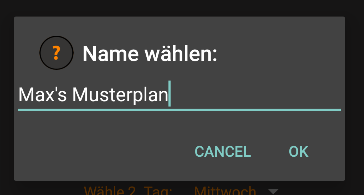
\includegraphics[scale=0.5]{img/plannameinput}
			\caption{Erfolgreiche Aktion: Trainingsplan generiert.}
		\end{subfigure}
	\end{figure}
	\subsubsection{Umsetzung des Algorithmus}
	Der Trainingsplan wird genau so wie in der Theorie beschrieben generiert. Je nach Trainingsziel bestimmt sich die Reihenfolge und Art der Trainingsphasen. Bei jeder Trainingsphase hat der Algorithmus einen bestimmten Übungspool zur Verfügung, die sich aus den Muskelgruppen und dem Schwierigkeitsgrad einer jeweiligen Übung erschließen. Die Anzahl der Wiederholungen \& Sätze variieren jeweils in dem angegeben Bereich in der Theorie, die sich in den Trainingsphasen unterscheiden. Der Algorithmus beachtet alle Bedingungen und verteilt die herangezogenen Übungen auf die angegebenen Trainingstage. 
	\ \\
	Je nach Dauer der Trainingsphase werden die Übungen eine bestimmte Anzahl an Wochen eingebracht. Die Summe der Dauer der Trainingsphasen ist die Dauer eines Trainingsplan, wodurch sich mittels Startdatum das Enddatum berechnen lässt. Nach jeder Trainigsphase folgt die Nächste, bis der Plan zu ende ist. 
\end{document}